\documentclass[12pt,lettersize,oneside]{article}
\usepackage[spanish]{babel}
\usepackage[utf8]{inputenc}
\usepackage{amsmath}
\usepackage{amssymb}
\usepackage{fancyhdr}
\usepackage{longtable}
\usepackage{sudoku}
\usepackage[hyphens]{url}
\usepackage{listings}
\lstset{
  language=C,
  basicstyle=\small
}
\usepackage[pdftex]{graphicx}
\usepackage{color}
\definecolor{gray75}{gray}{.75}
\lstdefinestyle{consola}
{basicstyle=\small\bf\ttfamily,
backgroundcolor=\color{gray75},
}
\lstdefinestyle{consola2}
{basicstyle=\footnotesize\bf\ttfamily,
backgroundcolor=\color{gray75},
}
\pagestyle{fancy}


\title{Grupo 3 \\Tercera versión de KECOSATS}
\author{Carlos Colmenares \and Kelwin Fernández \and Eleazar Leal}
\begin{document}
\maketitle
\setlength{\parskip}{2.5mm}
\setlength{\itemsep}{0ex }
%\tableofcontents
\section{Introducción}

\subsection{Motivación del proyecto}
En 1971, Stephen~Cook propuso en su trabajo\cite{Cook} una nueva categoría de
complejidad de problemas de decisión computacionales, a la que llamó problemas
\emph{NP-completos}. La caracterización de esta categoría se hace sobre estas
dos propiedades:
\begin{itemize}
  \item Todos los problemas \emph{NP-completos} pueden ser verificados en tiempo
    $O(p(n))$, donde $p(n)$ es un polinomio en función de $n$ el tamaño de la
    instancia del problema. 
  \item Todos los problemas en \emph{NP} pueden ser reducidos en tiempo
    $O(p(n))$ a algún problema \emph{NP-completo}, donde $p(n)$ es un polinomio
    en función de $n$ el tamaño de la instancia del problema que es reducido.
\end{itemize}

Ahora bien, fueron Cook y Leonid~Levin quienes encontraron, de forma
independiente, el primer problema en esta categoría \emph{NP-completos}: el
problema de la \emph{satisfacción booleana~(SAT)}. Un año después, Richard~Karp
identificó otros 21 problemas en esta categoría \cite{Karp}, los cuales tenían
la notoria característica de que para ellos no se conoce un algoritmo polinomial
(en función del tamaño de la instancia) que les dé solución, una cualidad que
comparten todos los problemas en esta clase, junto al hecho de que todos estos
problemas ocurren con una marcada frecuencia en el área de la computación. Sin
embargo, la característica más especial de éstos es el segundo ítem de arriba:
encontrar un algoritmo polinomial para tan sólo uno de ellos es encontrar un
algoritmo polinomial para todos.

De modo pues que una motivación para este proyecto estriba en el hecho de que
\emph{SAT} fue el primer problema que se demostró que pertenece a
\emph{NP-Completos} y que todos los problemas en esta clase son reducibles en
tiempo polinomial a él. Siendo así y bajo el supuesto de que estas reducciones a
\emph{SAT} se caractericen por polinomios de bajo grado y coeficientes pequeños,
cualquier mejora en tiempo que se pueda realizar a los algoritmos exponenciales
hoy conocidos para resolver el problema \emph{SAT} es una mejora para los
algoritmos exponenciales conocidos para los demás problemas en
\emph{NP-completos}.

Dejando por los momentos a un lado la discusión anterior sobre \emph{SAT},
haremos algunos comentarios sobre el conocido problema de \emph{Sudoku}, el cual
a primera vista, pareciera no estar vinculado al anterior. Este último ha
adquirido en los últimos años una gran notoriedad en el ámbito que ocupan otros
juegos como los crucigramas. Curiosamente, el problema \emph{Sudoku} comparte
con \emph{SAT} la peculiaridad de estar en \emph{NP-completos}. Este hecho hace
del \emph{Sudoku} un problema tanto difícil como interesante el cual tiene a su
vez otra característica: su naturaleza inherentemente gráfica que lo hace un
vehículo ameno para estudiar \emph{SAT}.

A continuación describiremos estos problemas, así como la relación entre ellos
con mayor detalle.

\subsection{Breve descripción del problema} 

El problema del \emph{Sudoku}, al cual queremos encontrar una solución
algorítmica ``eficiente'', consiste en lo siguiente:\vspace{-2.5mm}
\begin{enumerate}
\item La forma general de las instancias: Están dados un tablero de $N^2 \times
  N^2$ casillas, con $N\geq 3$. Este tablero está dividido en $N^2$ sub-tableros
  \emph{Sudoku} de $N \times N$ casillas, tal que estos sub-tableros no se
  solapan. Se da también con la instancia una colección $S$ de casillas de este
  tablero que ya han sido asignadas con valores en $V=\{1,2,\ldots,N^2\}$ tal
  que esta asignación preliminar $S$ a las casillas no viola ninguna de las
  reglas de \emph{Sudoku} que se enuncian más abajo. Ver la figura
  \ref{instanciaSudoku} para apreciar un ejemplo de instancia de \emph{Sudoku}
  $3 \times 3$.

\item La pregunta cuya respuesta se quiere determinar: ¿existe alguna asignación
  de enteros del conjunto $V=\{1,2,\ldots,N^2\}$ en las casillas del tablero
  restante ---las que no han sido asignadas en esta asignación preliminar ---,
  tal que se cumplan todas las condiciones siguientes?
    \begin{itemize}
    \item Por cada fila del tablero, cada entero en $V$ ocurre una y sólo una
      vez.
    \item Por cada columna del tablero, cada entero en $V$ ocurre una y sólo una
      vez.
    \item Por cada $N \times N$ sub-tablero \emph{Sudoku}, cada entero en $V$
      ocurre una y sólo una vez.
    \end{itemize}
    En caso de que exista tal asignación, se quiere saber cuál es. Véase la
    figura \ref{solSudoku} para apreciar una asignación que satisface a la
    instancia de \emph{Sudoku} que se propone en la figura
    \ref{instanciaSudoku}. 
\end{enumerate}
\begin{figure}\caption{Ejemplo de instancia de Sudoku para un tablero con $N=3$.}
\label{instanciaSudoku}
\setlength\sudokusize{6.5cm}
\begin{sudoku}
| |2| | |9|1| | | |.
|7| | | | | | |6| |.
| | |6| |7| |2|9|8|.
| | | |5|6| |3| | |.
| |5| |2| | | | | |.
|2| | | | | | | |4|.
|4|9|1| | |3| |8| |.
| | | | |2|8|1| | |.
| | |2| | | | | |7|.
\end{sudoku}
\end{figure}

\begin{figure}\caption{Ejemplo de asignación que satisface a la instancia de
    Sudoku propuesta en la figura \ref{instanciaSudoku}.}
\label{solSudoku}
\setlength\sudokusize{6.5cm}
\begin{sudoku}
|8|2|5|6|9|1|4|7|3|.
|7|4|9|3|8|2|5|6|1|.
|3|1|6|4|7|5|2|9|8|.
|1|7|8|5|6|4|3|2|9|.
|9|5|4|2|3|7|8|1|6|.
|2|6|3|8|1|9|7|5|4|.
|4|9|1|7|5|3|6|8|2|.
|6|3|7|9|2|8|1|4|5|.
|5|8|2|1|4|6|9|3|7|.
\end{sudoku}
\end{figure}

\vspace{-2.5mm}

\subsection{Estrategia para abordar el problema}

Como se demuestra en \cite{YatoSeta}, el problema de \emph{Sudoku} antes
descrito pertenece a la categoría NP-completos, de modo pues que hasta la fecha
no se conoce un algoritmo polinomial que lo resuelva. Asimismo, el hecho de que
este problema sea NP-completo implica que el problema de satisfacción booleana
\emph{SAT} es reducible en tiempo polinomial a él y viceversa. Más
concretamente, la siguiente formulación es una reducción polinomial del problema
\emph{Sudoku} a \emph{SAT}:

\rule{4cm}{0.3mm}

\textbf{Reducción polinomial de \emph{Sudoku} a \emph{SAT} }

La siguiente reducción polinomial ha sido adaptada de \cite{url}:
\vspace{-2.5mm}

\begin{itemize}
\item Para todo $i,j,d \in \{ 1,2,\ldots,N^2\}$, se definen las variables:

\[ x_{i,j}^d = \begin{cases} 1, & \mbox{si la casilla $(i,j)$ tiene el número
    $d$.} \\
    0, & \mbox{si no.} \end{cases}\]

\item Luego se consideran las siguientes cláusulas, clasificadas en 3 grupos:
\vspace{-2.5mm}

\begin{enumerate}
\item Cada casilla debe contener un número del $1$ al $N^2$.

     Para cada $i,j \in \{1,2,\ldots,N^2\}$ se tiene la cláusula:
       \[ x_{i,j}^1 \vee x_{i,j}^2 \vee \ldots \vee x_{i,j}^{N^2}.\]

\item Una casilla no puede tener dos números distintos asignados:

     Para cada $i,j \in \{1,2,\ldots,N^2\}$ se tiene la cláusula:
     \[ \bigwedge_{1\leq d < d' \leq N^2} (\neg x_{i,j}^d \vee x_{i,j}^{d'}).\]

\item Dos casillas distintas en una misma fila, columna o sub-tablero
  \emph{Sudoku} no pueden tener asignadas el mismo número:

     Si $x_1,x_2,\ldots, x_{N^2}$ representan las casillas de una fila, columna
     o sub-tablero dado, tendremos la siguiente cláusula:

     \[ \bigwedge_{d=1}^{N^2} \left( \bigwedge_{1\leq i < j \leq N^2}
       \left( \neg x_{i}^d \vee \neg x_{j}^{d} \right)\right).\]

\item Por último se agregan las asignaciones preliminares hechas a las casillas
  del \emph{Sudoku} y que por tanto forman parte de la instancia:

      Para cada $i,j \in \{1,2,\ldots, N^2\}$ si la casilla $(i,j)$ fue asignada
      ---de manera preliminar--- con el valor $d \in \{1,2,\ldots,N^2\}$, entonces
      se agrega la cláusula:

      \[ x_{i,j}^d= 1.\]
\end{enumerate}
\end{itemize}\vspace{-2.5mm}
\rule{4cm}{0.3mm}

Una vez presentada la anterior formulación de \emph{Sudoku} en términos de
\emph{SAT}, aclaramos que será esta reducción y no la inversa ---que no hemos
expuesto--- la que nos servirá de utilidad para intentar resolver el problema de
\emph{Sudoku}.

En virtud de que \emph{SAT} es un problema que ha sido estudiado con bastante
profundidad, se han propuesto numerosas heurísticas para acelerar el proceso de
búsqueda de soluciones. Es por ello que abordar \emph{Sudoku} con esta
estrategia que hemos descrito promete buenos resultados.

Una vez escogida esta estrategia para enfrentar el problema de \emph{Sudoku}, es
necesario entonces exponer también el problema \emph{SAT} al cual hemos
reducido el anterior. Para ello presentaremos un par de definiciones
preliminares y luego describiremos brevemente a \emph{SAT}.

 Llamaremos \emph{cláusula} a la disjunción de un conjunto finito de
variables booleanas, cada una de las cuales puede ocurrir con polaridad positiva
(no negada: $x_i$) o con polaridad negativa (negada $\overline{x_i}$).  Ejemplos
de cláusulas son: $(x_1 \wedge x_2)$, $(\overline{x_3})$, $(\overline{x_1}
\wedge x_3)$.

Una \emph{fórmula} es en cambio la conjunción de un conjunto finito de
cláusulas. Por ejemplo: $F_1:\ (x_1 \vee x_2 \vee \overline{x_3}) \wedge (x_1
\vee \overline{x_2}) \wedge (\overline{x_3})$ es una cláusula.

El \emph{problema de la satisfacción booleana~(SAT)} consiste de la
forma general de las instancias al problema y de la pregunta: \vspace{-2.5mm}
\begin{enumerate}
\item La forma general de las instancias: Dados un conjunto finito de variables
  booleanas $x_1,x_2,\ldots,x_n$ y una fórmula booleana $F(x_1,x_2,\ldots,x_n)$
  en forma normal conjuntiva (CNF).
\item La pregunta cuya respuesta se quiere determinar: ¿existe una asignación de
  valores de verdad a las variables $x_1,\ldots, x_n$ tal que la fórmula sea
  verdad? En caso de que exista tal asignación, se quiere saber cuál es.
\end{enumerate}

De aquí en adelante, concentraremos nuestra atención en el problema de
\emph{satisfacción booleana}.

\subsection{Descripción del contenido del informe}
En el presente reporte se expondrán los algoritmos y tipos de datos
fundamentales empleados por el programa KECOSATS para decidir el problema de la
satisfacción booleana. Asimismo, se presentarán las decisiones de diseño que
orientaron la implementación del mismo.

\section{Diseño}

\subsection{Descripción general del algoritmo empleado}
El programa propuesto sigue el esquema general del algoritmo DPLL que presentaron
Martin Davis, Hilary Putnam, George Logemann y Donald Loveland para decidir el
problema de satisfacción booleana.

Seguidamente presentamos el esquema general del algoritmo DPLL, que hemos
adaptado de \cite{Zhang}:

\begin{lstlisting}
  status = preprocess(); 
if (status != UNKNOWN) return status; 
while(true) { 
  // Fase de seleccion de variable a asignar.
  decide_next_branch(); 
  while (true) { 
    // Fase de deduccion.
    status = deduce(); 
    if (status == CONFLICT) { 
      conflict_result = analyze_conflict(); 
      if (conflict_result == 0) 
        return UNSATISFIABLE; 
      else backtrack(conflict_result); 
    } 
    else if (status == SATISFIABLE) 
      return SATISFIABLE; 
    else break; 
  } 
 } 
\end{lstlisting}
\vspace{-2.5mm}

En esta versión del programa KECOSATS que aquí describimos, se realiza el
análisis de conflictos, el cual permite detectar las causas de los mismos, que
unido al aprendizaje de cláusulas hace posible que se puedan descartar grandes
secciones del espacio de búsqueda a través de la ejecución del
\emph{backtracking} no cronológico: aquel que frente a conflictos puede
retroceder, no sólo al nivel inmediatamente anterior, sino que puede retroceder
dando saltos de longitud mayor a 1, con base en un estudio de la naturaleza del
conflicto.

Entre las razones por las que se escogió el algorimo DPLL están:
\begin{enumerate}\vspace{-2.5mm}
\item Este algoritmo es la base para las implementaciones de los
  \emph{SAT-solvers} completos ---no estocásticos--- más eficientes conocidos.
\item El esquema general del algoritmo es bastante sencillo de implementar como
  de comprender.
\end{enumerate}
\subsection{Fase de selección de variables a asignar}\label{ProxVariable}

En esta tercera versión de KECOSATS se ha incorporado una nueva heurística de
selección de la variable que se va a asignar. Esta heurística es la que ha sido
propuesta por Goldberg y Novikov en el trabajo \cite{goldberg} y que está
incorporada en el programa \emph{BerkMin}.

\subsubsection{Descripción de la heurística de BerkMin}\label{TeoHeur}
\footnote{En esta sección se tratan algunas nociones que serán descritas más
  adelante, así que el lector pudiera omitir esta sección en una primera
  lectura.}La heurística de \emph{BerkMin} busca seleccionar como variables para
asignar aquella que ha tenido mayor participación o actividad en los conflictos
recientes. Por esta razón, es necesario contar con una forma de estimar tal
actividad para cada una de las variables del problema. Para ello, cada variable
$x_i$ tiene asignado un contador $ac(x_i)$ que almacena una aproximación al
número de cláusulas inducidas por conflictos\footnote{La noción de cláusula
  inducida por conflicto es presentada más adelante en la sección
  \ref{analisisConflicto}.} en los que aparece un literal $x_i$ o
$\overline{x_i}$, correspondiente a la variable $x_i$.

Hemos mencionado que se almacena una \emph{aproximación} por dos razones:
\vspace{-2.5mm}
\begin{enumerate}
\item Como la intención es seleccionar la variable de mayor actividad
  \emph{reciente}, periódicamente hay que ir restando importancia a los valores
  de actividad de variables cuya  participación ha sido ya hace un tiempo. La
  forma como \emph{BerkMin} y \emph{zChaff} implementan esto es dividiendo los
  valores $ac(x_i)$ por constantes pequeñas cada cierto tiempo.
\item La heurística de \emph{BerkMin}, a diferencia de la de \emph{zChaff}, no
  sólo incrementa el valor $ac(x_i)$ cuando algún literal de $x_i$ ocurre en la
  cláusula inducida por conflicto $\kappa$. Sino que también lo incrementa si
  $x_i$ es una variable deducida y no asignada que se encuentra en el grafo de
  implicaciones que termina en el conflicto $\kappa$ y que por tanto, es
  alcanzable desde el nodo $\kappa$ en el recorrido en profundidad en reverso
  que se realiza en la fase de análisis de conflicto.
\end{enumerate}

Ahora bien, para seleccionar la variable a asignar, se examina la última
cláusula aprendida y de las variables asociadas a literales que ocurran en esta
cláusula se escoge la que tenga el mayor valor $ac(x_i)$ y que no esté
asignada. Si no hay una variable que no está asignada o si no hay cláusula
aprendida, se escoge aquella variable, de entre \emph{todas} las variables del
problema, que no esté asignada y que tenga el máximo valor $ac(x_i)$.

Una vez que se ha descrito el mecanismo que permite aproximar la actividad
reciente de las variables, queda el problema de determinar cuál valor de verdad
o falsedad asignar a la variable seleccionada. Para ello \emph{BerkMin} propone
un contador adicional $ac\_lit(x_i) \in \mathbb{Z}$ para ayudar a discernir cuál
es el valor de verdad ``más prometedor'' que se puede asignar a $x_i$.

La forma como que actualiza el contador es la siguiente: El contador
$lit\_ac(x_i)$ es incrementado en 1 cada vez que se genera una nueva cláusula
inducida por conflicto en la que ocurre el literal $x_i$ (con polaridad
positiva) y decrementado en 1 cada vez que se genera una nueva cláusula inducida
por conflicto en la que ocurre el literal negado $\overline{x_i}$. Para
seleccionar cuál valor de verdad asignar a la variable escogida, se examina
$lit\_ac(x_i)$. Si el valor es positivo, entonces se escoge la polaridad
positiva. Si es negativo, se escoge la polaridad negativa. Si es nulo el valor,
se escoge cualquier polaridad.

Como desventaja de esta heurística está que en el peor caso, habrá que recorrer
la lista completa de variables para encontrar tanto aquella variable que tiene
mayor actividad reciente.


% En principio, si el
% \emph{backtracking} fuera cronológico y no hubiera aprendizaje de cláusulas,
% la selección de var 

% Esta heurística es razonable porque las variables cuyos literales han aparecido
% recientemente con mayor frecuencia en las cláusulas inducidas por conflicto,


\subsubsection{Descripción de la heurística de KECOSATS}

KECOSATS propone también una heurística propia que guarda alguna relación con
la heurística de la primera versión de KECOSATS. Para la selección de la próxima
variable no asignada, a la que se le dará un valor booleano. La heurística
KECOSATS mantiene el cálculo de la actividad reciente de cada variable $x_i$ en
el contador $ac(x_i)$. Así que el plan para escoger la variable a asignar
funciona tal cual como lo sugiere la heurística de \emph{BerkMin}. 

Las diferencias entre la heurística \emph{BerkMin} y KECOSATS son:\vspace{-2.5mm}
\begin{enumerate}
\item Al momento de decidir cuál valor de verdad dar a la variable seleccionada
  para asignar $x_i$, se adopta esta estrategia: 

  Si el número de cláusulas en las que ocurre el literal negado $\overline{x_i}$
  es mayor que el número de cláusulas en las que ocurre no negado $x_i$
  entonces, se decide asignar a la variable $x_i$ el valor falso. En caso
  contrario, se le asigna a $x_i$ un valor de verdad.

\item Antes de comenzar a resolver el problema, la heurística \emph{BerkMin}
  asigna a los contadores $ac(x_i)$ el valor inicial 0. La heurística KECOSATS,
  en cambio, da a estos contadores unos valores iniciales fijos.
\end{enumerate}

La ventajas de haber escogido esta heurística son las siguientes:
\begin{enumerate}\vspace{-2.5mm}
\item En la mayoría de las instancias de pequeño tamaño en las que se probó esta
  heurística, se redujeron los tiempos de ejecución del programa. Asimismo, al
  menos 1 de los problemas \emph{Sudoku} de las 60 instancias que no era
  resuelto en menos de 50 segundos con la heurística de la segunda versión, pudo
  ser resuelto con esta nueva heurística en un tiempo mucho más razonable.
\item La forma de escoger el valor a asignar a la variable, antes descrita,
  sugiere que pudiera ser más probable que se detecten con mayor rapidez los
  conflictos ---en caso de que los hubiera.
\item Se trata de una heurística muy sencilla de comprender e implementar.
\end{enumerate}

Como desventaja de esta heurística está que en el peor caso, habrá que recorrer
la lista completa de variables para encontrar aquella variable que tiene mayor
actividad reciente. Tal como se ha mencionado, esta desventaja la comparten las
heurísticas \emph{BerkMin} y KECOSATS.

\subsection{Fase de deducción}

Una vez que se ha seleccionado una variable para asignar junto al valor que se
le asignará, se inicia la fase de deducción del algoritmo DPLL. Es en esta fase
que se procede a la identificación y propagación de cláusulas unitarias. En esta
sección describiremos los algoritmos de propagación de restricciones booleanas y
de identificación y eliminación de literales puros.


\subsubsection{Identificación y propagación de cláusulas
  unitarias}\label{UnitPropagation}
Tal como se indica en \cite{Zhang} y \cite{ZhangThesis}, el estudio de
implementaciones del algoritmo DPLL que se han realizado con el pasar de los
años, sugiere que la propagación de cláusulas unitarias como mecanismo de
deducción parece ser el más eficiente que se ha encontrado hasta ahora.

La \emph{propagación de cláusulas unitarias} consiste en ubicar cuáles cláusulas
de la fórmula ---dada ésta en forma normal conjuntiva--- están compuestas de un
solo literal. Estas cláusulas son llamadas \emph{cláusulas unitarias} y se
satisfacen con asignar a éste único literal el valor de verdad correspondiente.
Lo explicamos con un ejemplo: En la fórmula $F_1:\ (x_1 \vee x_2 \vee
\overline{x_3}) \wedge (x_1 \vee \overline{x_2}) \wedge (\overline{x_3})$, la
única cláusula unitaria es $\overline{x_3}$. Si se asigna $x_3:=0$, queda la
nueva fórmula $F_2:\ (x_1 \vee x_2 \vee \overline{x_3}) \wedge (x_1 \vee
\overline{x_2}) $ y bajo el supuesto de que $x_3=0$ se tiene que $F_2$ es
satisfactible si y sólo si $F_1$ lo es.

Para la identificación y propagación de cláusulas unitarias se escogió la
implementación de la propagación de cláusulas unitarias con 2 testigos por
cláusula, que es referida por las fuentes (\cite{Zhang} y \cite{ZhangThesis} con
el nombre de \emph{2-watched literals}). Central en la idea de los
\emph{2-watched literals} es el concepto del \emph{watcher} o testigo: Dada una
cláusula, se asocian a ella 2 apuntadores, cada uno apunta a un literal que
ocurre en la misma cláusula. Estos apuntadores son lo que se conocen con el
nombre \emph{watchers}.

Los \emph{2-watched literals} es la implementación empleada por \emph{zChaff} y 
en ella se asocia a cada literal $x_i,\ i\in{1,\ldots,n}$ un par de listas, la
primera de ellas tiene como elementos a todas las cláusulas en las que la el
literal $x_i$ ocurre no negado (polaridad positiva) como testigo o \emph{watched
  literal}. La segunda lista asociada a $x_i$ tiene como elementos a todas las
cláusulas en las que el literal $\overline{x_i}$ ocurre como testigo o
\emph{watched literal}.

Asimismo reiteramos por motivo claridad, que cada cláusula tiene asociados dos
apuntadores a literales que ocurren dentro de ella, estos apuntadores son los
\emph{watchers} a los que nos hemos referido antes.

Ahora bien, para detectar si, tras asignar $x_i=0$, una cláusula
es unitaria se buscan todas las cláusulas en las que aparezca $x_i$ con
polaridad positiva (no negada) y como \emph{watcher}. Este último apuntador debe
ser movido a otro literal no asignado en la misma cláusula. Si el único literal
no asignado en esa cláusula está siendo apuntado por el otro \emph{watcher}
entonces esa cláusula es unitaria. 

Para la implementación de este mecanismo de deducción, se escogió la
implementación de los \emph{2-watched literals} descrita en las fuentes
\cite{Marques}, \cite{Zhang} y \cite{ZhangThesis} y que fue propuesta con el
programa \emph{Chaff}.

% Seguidamente describiremos someramente la implementación \emph{2-watched
%   literals} para la detección de cláusulas unitarias. Sin embargo, referimos al
% lector a los trabajos \cite{Marques}, \cite{Zhang} y \cite{ZhangThesis} para una
% explicación más detallada.


Las razones para escoger esta implementación de \emph{2-watched literals} para
la identificación de cláusulas unitarias son las siguientes:\vspace{-2.5mm}
\begin{enumerate}
\item En pruebas de ejecución\cite{Zhang} se ha observado que el comportamiento
  de la implementación por \emph{2-watched literals} requiere de menor tiempo
  que implementaciones como la de \emph{SATO} ---implementación a la que
  \cite{Zhang} se refiere como \emph{Head/Tail lists}--- y considerablemente
  menor tiempo que la implementación por contadores.
\item La implementación de \emph{2-watched literals} no requiere que se realicen
  operaciones sobre los \emph{watchers}, o sobre el conjunto de datos que
  permite directamente determinar cuáles son las cláusulas unitarias, cuando se
  realiza el \emph{backtracking} a un nivel de decisión anterior. Las
  implementaciones de \emph{SATO} y contadores sí requieren estas
  operaciones. Esta ventaja es señalada por el trabajo \cite{Marques}.
\end{enumerate}

Entre las desventajas que trae consigo la implementación de \emph{2-watched
  literals} está:\vspace{-2.5mm}
\begin{enumerate}
\item Cuando es necesario mover alguno de los \emph{watchers}, porque la variable
  a la que apuntan en la cláusula resulta asignada, se debe buscar una nueva
  variable no asignada---puede que ni exista tal variable--- en la misma
  cláusula. Entonces, en el peor caso, para identificar una cláusula unitaria,
  la implementación de \emph{2-watched literals} tendrá que \emph{recorrer todos
    los literales de una misma cláusula} en busca de esta variable no asignada.
\end{enumerate}



\subsubsection{Eliminación de literales puros}

La \emph{eliminación de literales puros} en una fórmula dada en forma normal
conjuntiva consiste en ubicar primero cuáles son las variables booleanas que
sólo ocurren con una polaridad en la fórmula. Ahora bien, estos literales que
ocurren con una única polaridad en toda la fórmula no condicionan la
satisfacción de la fórmula; es decir, si se eliminaran todos los literales
puros, la fórmula resultante es satisfactible si y sólo si asignando a los
literales puros los valores de verdad que los satisfagan, se logra que la
fórmula original lo sea. Lo explicamos con un ejemplo: En la fórmula siguiente
$F_1:\ (x_1 \vee x_2 \vee \overline{x_3}) \wedge (x_1 \vee \overline{x_2})
\wedge (\overline{x_3})$ el único literal puro es $x_1$, de forma que $F_1$ será
satisfactible si y sólo si asignando a $x_1$ el valor de verdad se logra que
$F_2:(\overline{x_3})$ sea satisfecha.

Las implementación de este mecanismo deducción es bastante sencilla. Por tal
razón decidimos que no es necesario ahondar mucho más al respecto y pasamos de
inmediato a describirla. Para la implementación de la eliminación de literales
puros se hizo un recorrido por todas las cláusulas de la fórmula anotando cuál
es la polaridad que se ha observado para cada literal. Si en un momento del
paseo por las cláusulas de la fórmula se encuentra con un literal que ocurre con
una polaridad distinta a la ya observada anteriormente para ese literal, se
descarta que esa variable sea un literal puro.

Entre las desventajas que acarrea esta implementación de la \emph{eliminación de
literales puros} está:\vspace{-2.5mm}
\begin{enumerate}
\item Un elevado costo en tiempo del programa, por cuanto implica un recorrido
  por todos los literales de todas las cláusulas de la fórmula.
\end{enumerate}\vspace{-2.5mm}
\subsection{Fase de análisis del conflicto}\label{analisisConflicto}

Esta fase de KECOSATS consiste de la identificación de las causas necesarias y
suficientes para un dado conflicto, con los siguiente objetivos: evitar este
mismo conflicto más adelante e implementar el \emph{backtracking no
  cronológico}.  Ahora daremos unas definiciones preliminares necesarias para
discutir el grafo de implicaciones, estructura vital para el análisis de
conflictos.

% Una vez que KECOSATS se encuentra con una situación conflictiva producto de las
% decisiones de asignación que ha tomado ---y tras la propagación de éstas con la
% propagación de cláusulas unitarias---, éste busca un camino alternativo en la
% arborescencia implícita del \emph{backtracking} para tratar así de dar con
% alguna solución al problema de satisfacción, en caso de que exista. No
% ahondaremos por ahora en detalle sobre esta arborescencia implícita, porque se
% discutirá más adelante. 


Durante la ejecución de KECOSATS, se asigna a cada variable que se decide $x_i$
un nivel de decisión $\delta$; esto es un entero mayor que 1 que comparte $x_i$
con todas las variables unitarias que son propagadas a consecuencia de la
asignación de $x_i$ y que no comparte con ninguna otra variable. El nivel de
decisión de manera incremental y la primera variable $x_1$ que decide el
programa tiene asociado un $\delta(x_1) =1$ al igual que todas las variables
unitarias que son propagadas tras asignar $x_1$. Luego se decide la variable
$x_2$ a la que se le asigna $\delta(x_2)=2$ y así sucesivamente.

Una definición que en gran medida simplificará la discusión del grafo de
implicaciones es el de las asignaciones antecedentes de una variable y
asociadas a un cláusula. Dada la variable $x$ que ocurre como literal ---bien
sea como $\overline{x}$ o $x$--- en la cláusula $\omega = v_1 \vee v_2 \vee
\ldots \vee x \vee \ldots v_n$ del problema, el conjunto de \emph{asignaciones
  antecedentes} de $x$, escrito $A(x)$, asociadas a la cláusula $\omega$ es
la colección de asignaciones a variables $v_i \neq x,\ i \in \{1,2,\ldots n\}$
que son directamente responsables de que $x$ sea unitaria en $\omega$.

\subsubsection{Grafo de implicaciones}
Para el análisis del conflicto, KECOSATS adopta una estrategia introducida por
Silva y Sakallah en GRASP y por Bayardo y Schrag. \'Esta consiste en armar
durante la ejecución del \emph{solver} un \emph{grafo de implicaciones} $G$
definido como sigue\footnote{Esta definición se adaptó de \cite{grasp96}.}:
\begin{itemize}\vspace{-2.5mm}
\item Todos los vértices de $G$ son asignaciones de un valor booleano $v(x_i)
  \in \mathbb{B}$ a una variable $x_i$ del problema.
\item Los predecesores en $G$ de una asignación $x_i \gets v(x_i)$ son todas las
  asignaciones antecedentes $A(x_i)$ que están asociadas a la cláusula $\omega$
  que forzó a $x_i$ a ser asignada por propagación ---porque $x_i$ resultó
  unitaria en $\omega$. Los lados de los predecesores hacia la asignación $x_i
  \gets v(x_i)$ se etiquetan con la cláusula $\omega$.
\item Se agregan unos vértices especiales que denotan los conflictos. Cada
  conflicto consiste de una cláusula $\omega$ del problema que es falsa bajo las
  asignaciones hechas. Siendo así, los predecesores de un conflicto son las
  asignaciones a las variables en $\omega$ que obligaron a que ésta fuera
  falsa. Los lados que provienen de los predecesores del conflicto asociado a la
  cláusula $\omega$ están todos etiquetados con $\omega$.
\end{itemize}\vspace{-2.5mm}

La utilidad de este grafo de implicaciones es \emph{permite identificar
  asignaciones necesarias y suficientes para que se produzca un conflicto dado}
obteniendo de ello dos beneficios:
\begin{itemize}
\item A partir de esas condiciones necesarias se puede construir una cláusula
  redundante ---que no altera la satisfactibilidad del problema original--- que
  se puede agregar a una base de datos de cláusulas y evitar en el futuro que
  aparezca el mismo conflicto.
\item A partir de las asignaciones necesarias para que se produzca el conflicto,
  es posible calcular el mayor nivel de decisión $\delta_{max}$ de todas
  ellas. Hacer \emph{backtracking} a cualquier nivel de decisión mayor que
  $\delta_{max}$ producirá el mismo conflicto por las características de estas
  asignaciones que hemos dicho que son calculables a partir del grafo de
  implicaciones. Entonces para evitar este conflicto, el \emph{backtracking}
  debe realizarse hasta el nivel de decisión $\delta_{max}$, que corresponde al
  nivel en que se realizó la última de estas asignaciones necesarias y
  suficientes para este conflicto. Si se procede de este modo, se estaría
  implementando el \emph{backtracking no cronológico}, logrando entonces con
  ello reducir el espacio de búsqueda.
\end{itemize}

Es claro que cada vez que se realiza un paso de \emph{backtracking}, parte del
grafo de implicaciones debe deshacerse para reflejar el nuevo nivel de decisión
actual.
\subsubsection{Cláusula inducida por conflicto y aprendizaje}

Como hemos indicado, una vez que durante la ejecución de KECOSATS se presenta un
conflicto, el grafo de implicaciones permite obtener un conjunto de asignaciones
necesarias y suficientes para producir el anterior. La manera como se hace esto
es la siguiente:
\begin{itemize}
\item Partiendo del nodo conflicto en el grafo de implicaciones se hace un
  recorrido hacia sus predecesores hasta encontrar los nodos raíces: Para fijar
  ideas, digamos que para un dado conflicto, éste tiene como nodos raíces en el
  grafo de implicaciones a las asignaciones: $x_1 \gets 1$ con nivel de
  decisión 2 y $x_3 \gets 0$ con nivel de decisión 5. Ello quiere decir que
  cada vez que se haga este par de asignaciones y se haga la propagación de las
  cláusulas unitarias nos encontraremos con el mismo conflicto.

\item Una vez identificadas estas asignaciones raíces, se construye una nueva
  cláusula $x_i^{v(x_i)}$ para toda variable $x_i$ en estas asignaciones raíces
  encontradas anteriormente en el recorrido sobre el grafo de implicaciones
  antes descrito y donde $x_i^0= x_i$ y $x_i^1=\overline{x_i}$. En el caso anterior,
  la cláusula nueva que se construye sería $x_1^{1} \vee x_3^{0}$ que sería
  $\overline{x_1} \vee x_3$. Estas cláusulas construidas a partir de un conflicto se
  conocen como \emph{cláusulas inducidas por conflicto} y son redundantes con el
  conjunto original de cláusulas de la instancia, en el sentido en que agregar
  estas cláusulas inducidas por conflicto al conjunto inicial de cláusulas no
  altera la satisfactibilidad de la instancia. El aprendizaje consiste entonces
  en incluir estas cláusulas inducidas por los conflictos en una base de datos
  de cláusulas, con el objetivo de prevenir que la misma asignación conflictiva
  ocurra más adelante en el transcurso de la ejecución del algoritmo sobre una
  instancia.
\end{itemize}

Hemos mencionado brevemente cómo analizar los conflictos con la ayuda de un
grafo de implicaciones con un ejemplo muy sencillo que implicaba asignaciones a
$x_1$ y $x_3$. Consideramos conveniente para una descripción más detallada del
proceso de búsqueda de las cláusulas inducidas por conflicto recomendar al lector
que consulte además las fuentes \cite{grasp96} y \cite{ZhangThesis}, en donde se
presentan algunos ejemplos más elaborados.

\subsubsection{Backtracking no cronológico}
Como mencionamos anteriormente, el proceso de determinación de las cláusulas
inducidas por conflicto permite además implementar el \emph{backtracking no
  cronológico}. Esto es porque una vez determinada la cláusula inducida por
conflicto, que en el ejemplo anterior era $\overline{x_1} \vee x_3$, y
conociendo los niveles de decisión de las asignaciones a estas variables se
tiene a cuál nivel hay que retroceder en el \emph{backtracking}: basta tomar el
máximo de los niveles de decisión de cada variable que ocurre en la cláusula
inducida por el conflicto. En el ejemplo propuesto este máximo sería 5 ---el
nivel de decisión en que se asignó $x_3 \gets 0$. Haciendo el
\emph{backtracking} hasta este nivel permitiría descartar grandes secciones del
espacio de búsqueda, porque regresando a cualquier nivel de decisión $>5$ se
producirá el mismo conflicto.
% Tal situación conflictiva consiste de al menos una cláusula $C=
% \overline{x_5},\overline{x_6}$ del problema que no es satisfecha con la
% asignación parcial que se ha construido hasta el momento


\section{Implementación}

El programa que proponemos está orientado por los cambios que se realizan,
durante la ejecución, sobre una variable global de nombre {\tt sat\_st} que es la
única con el tipo {\tt SAT\_status} en todo el programa. 
Este tipo de dato registra: \vspace{-4.5mm}
\begin{enumerate}
\item La información que es necesario preservar de la instancia del problema de
  satisfacción que se ha leído y que se pretende resolver.
\item El estatus de resolución de un problema de satisfacción en cualquier
  momento dado.
\end{enumerate}
Por esta razón podríamos afirmar que este es el tipo de dato más importante de
todo el programa.
Presentamos ahora la definición del tipo {\tt SAT\_status}
\begin{lstlisting}
typedef struct SAT_status{    
    int num_vars;
    int num_clauses;
    clause *formula;
    list *pos_watched_list;
    list *neg_watched_list;
    stack backtracking_status;
    int *model;
    decision_node *impl_graph;
    double *ac;
    int *lit_ac;                     
} SAT_status;
\end{lstlisting}
, para comentar sus campos con detalle:\vspace{-2.5mm}
\begin{itemize}
\item El atributo {\tt formula}, representa la fórmula en forma normal
  conjuntiva. Se trata de un arreglo de cláusulas, cada una de tipo {\tt
    clause}.
\item En la implementación que aquí se describe, se optó por por los campos {\tt
    pos\_watched\_list} y {\tt neg\_watched\_list} en el tipo {\tt
    SAT\_status}. Cada uno de éstos es un arreglo de cabezas de listas, de forma
  que {\tt pos\_watched\_list[i]} sea la cabeza de la lista cuyos elementos son
  las cláusulas en las que el literal $x_i$ ocurre como
  \emph{watcher}. Análogamente ocurre con {\tt neg\_watched\_list[i]}: es la
  cabeza de la lista cuyos elementos son las cláusulas en las que el literal
  $\overline{x_i}$ ocurre como \emph{watcher}.

\item El campo {\tt model} del tipo {\tt SAT\_status} es un arreglo de enteros
  tal que {\tt model[i]} es el valor de asignación que se prueba para la
  variable $x_i$. El {\tt model} indica cuál nodo de la arborescencia del
  \emph{backtracking} se está considerando en un determinado instante de la
  ejecución\footnote{Véase la sección \ref{backtracking} que describe la
    arborescencia implícita que se recorre en el \emph{backtracking}.}.

\item Se incluye el campo {\tt num\_clauses} en el tipo {\tt SAT\_status}, para
  poder recorrer el arreglo {\tt formula} de todas las cláusulas que componen la
  fórmula.

\item El campo {\tt impl\_graph} es un arreglo de longitud igual al número de
  variables booleanas del problema: {\tt sat\_st.num\_vars}, el cual modela el
  estado del grafo de implicaciones en un momento dado. Seguidamente
  describiremos un poco más este campo con un ejemplo:

  Si la variable $x_i$ se encuentra asignada en un momento dado de la ejecución,
  tal asignación pudo haber sido de decisión o de implicación. Si fue de
  implicación, entonces hay alguna cláusula unitaria $\omega$ cuyo único literal
  unitario es $x_i$ o $\overline{x_i}$. En este caso, {\tt impl\_graph[i]}
  contiene un apuntador a la cláusula $\omega$ que forzó la asignación implicada
  de $x_i$ y su nivel de decisión. Si la asignación de $x_i$ fue de decisión, el
  apuntador a esta cláusula es nulo y además se conserva también el nivel de
  decisión de $x_i$ en {\tt impl\_graph[i]}.

\item El campo {\tt ac} es un arreglo de longitud igual al número de variables
  de la instancia que se está resolviendo y contiene en la posición $i$ a un
  número de doble precisión que mide la actividad reciente que ha tenido la
  variable $x_i$. La idea es que las variables que hayan tenido mayor actividad
  reciente sean seleccionadas por el procedimiento {\tt decide\_next\_branch}
  para ser asignadas. Este arreglo se describe con mayor detenimiento en la
  sección de implementación de la heurística de selección de variable a asignar.
  Para más detalles consultar las secciones \ref{heur} y \ref{impl}.

\item El campo {\tt lit\_ac} es también un arreglo que tiene una longitud igual
  al número de variables del problema. Esta estructura apoya igualmente al
  procedimiento de selección de la próxima variable a asignar. Su tarea es
  concretamente medir cuál valor, de verdad o falsedad, asignar a la variable
  escogida para asignar en el {\tt decide\_next\_branch}.
\end{itemize}\vspace{-2.5mm}

A continuación comentaremos algunos detalles sobre la variable global {\tt
  sat\_st}. La razón por la que se escogió a {\tt sat\_st} de tipo {\tt
  SAT\_status} como variable global, en lugar de pasarla como parámetro entre
las sucesivas llamadas a funciones durante la ejecución del algoritmo son:
\begin{enumerate}
\item El pasaje del parámetro {\tt sat\_st} a cada una de las funciones supone
  un costo acumulado muy grande a lo largo de la ejecución de todo el
  programa. Cuando bien pudiera ahorrarse la operación de empilar esa parámetro
  en cada llamada.
\item Si se pasara una referencia a {\tt sat\_st} como parámetro a cada función,
  se incurriría en un costo adicional, en comparación con la alternativa de
  tener a {\tt sat\_st} como variable global, por la indirección que es
  necesario ejecutar en cada subrutina por cada vez que se quiera acceder a los
  campos de esta variable.
\end{enumerate}

\subsection{Implementación de las cláusulas}\label{clausulas}

Para la implementación de cada cláusula se definió el siguiente tipo de dato
{\tt clause}:
\begin{lstlisting}
typedef struct clause{
    int size;
    variable* head_watcher;
    variable* tail_watcher;
    variable* literals;
} clause;
\end{lstlisting}
, que a continuación describiremos campo por campo.\vspace{-2.5mm}
\begin{enumerate}
\item Los apuntadores {\tt head\_watcher} y {\tt tail\_watcher} señalan cuáles
  son los literales testigos ---\emph{watched literals}--- de una cláusula. En
  virtud de que en la fase de propagación de restricciones booleanas se optó por
  implementar la propagación de cláusulas unitarias con los \emph{2-watched
    literals} según se describe en \cite{Zhang},
  cada cláusula exige dos apuntadores a variables en la misma cláusula.

\item Como cada cláusula es una disjunción de literales, optamos por
  representarla como un arreglo de variables llamado {\tt literals}. Para poder
  recorrerlo es necesario almacenar su tamaño, que estará almacenado en el campo
  {\tt size} de la cláusula.
\end{enumerate}

\subsubsection{Ventajas de la implementación escogida para las cláusulas}
La implementación de los literales que componen una cláusula en un arreglo de
variables apuntado por {\tt literals} implica: \vspace{-2.5mm}
\begin{itemize}
\item Una rapidez de acceso en tiempo constante a cada literal de la
  cláusula. Hecho que resulta de particular utilidad en los recorridos a través
  de los literales de cada cláusula que son efectuados durante la detección de
  literales puros y durante la actualización de los \emph{watchers} o testigos
  que permiten identificar cláusulas unitarias. 

  Recuerde el lector que se ha mencionado en la sección \ref{UnitPropagation} que
  una de las desventajas de las implementación por \emph{2-watched literals} es
  que en el peor caso hay que recorrer todos los literales de una cláusula para
  determinar si ésta es unitaria o no.

\item Un ahorro de espacio para los apuntadores, el cual sería necesario si la
  conjunción de literales en las cláusulas se implementara con una lista
  enlazada.
\end{itemize}


\subsection{Implementación del \emph{Backtracking}}
\subsubsection{\'Arbol implícito del \emph{Backtracking}}\label{backtracking}
Toda implementación de \emph{Backtracking} es un recorrido \emph{Depth-First
  Search} sobre una arborescencia implícita. Esta descripción implícita de la
arborescencia a recorrer exige que se defina cuáles son sus nodos y para cada
nodo, cuáles son sus nodos sucesores. En el caso que nos concierne, los nodos
son de la forma:
\[[x_{i_1}=\mathbb{B},x_{i_2}=\mathbb{B},\ldots, x_{i_k} = \mathbb{B} ], \]
donde $0\leq k \leq n$, con $n$ el número de variables de la instancia del
problema de satisfacción a resolver y $x_{i_k}=\mathbb{B}$ indica que la
variable booleana $x_{i_k}$ tiene un valor booleano (sea $1$ ó $0$)
asignado. Imponemos adicionalmente una condición a los nodos de esta
arborescencia y es que la asignación hecha a las variables del nodo:
$x_{i_1},\ldots,x_{i_k}$ \emph{no haga que la fómula no se pueda
  satisfacer}. Las $x_{i_k}$ denotan variables booleanas distintas $\forall k
\in \{1,\ldots,n\}$.

Ahora, dado un nodo $[x_{i_1}=\mathbb{B},x_{i_2}=\mathbb{B},\ldots, x_{i_k} =
\mathbb{B} ]$ sus sucesores son todos los nodos de la forma:
$[x_{i_1}=\mathbb{B},x_{i_2}=\mathbb{B},\ldots, x_{i_k} = \mathbb{B},
x_{i_{k+1}}=\mathbb{B} ]$.

El \emph{backtracking} implementado busca encontrar en la arborescencia ---en
caso de que exista--- un nodo de la forma
\[[x_{1}=\mathbb{B},x_{2}=\mathbb{B},\ldots, x_{n} = \mathbb{B} ], \] y que se
corresponde con una asignación de valores de verdad a todas las variables que
hace que la fórmula dada sea satisfecha ---si $n$ es el número total de
variables booleanas.
\vspace{-2.5mm}

\subsubsection{Estructuras de datos que apoyan la implementación del \emph{bactracking}}
El \emph{backtracking} se implementó iterativo en lugar de recursivo, por los
motivos que se señalan en la sección \ref{VentajasBacktracking}. Para ello fue
necesario trabajar explícitamente con una pila de elementos de un nuevo tipo de
dato llamado {\tt decision\_level\_data}. Este tipo almacena la información que
caracterizan a cada nodo del árbol implícito que se recorre en el
\emph{backtracking}\footnote{En \cite{Zhang} les llaman niveles de decisión.} y
que deben ser conservados en caso de que el algoritmo se encuentre con un nodo
parcial que no tiene sucesores; esto es, con un nodo
$[x_{i_1}=\mathbb{B},x_{i_2}=\mathbb{B},\ldots, x_{i_k} = \mathbb{B} ]$, $k< n$
tal que la asignación de cualquier otra variable no logra satisfacer la fórmula.

Presentamos entonces el tipo {\tt decision\_level\_data}:

\begin{lstlisting}
typedef struct decision_level_data{
    variable assigned_literal;
    int missing_branch;                                                
    list propagated_var;
} decision_level_data;
\end{lstlisting}
que a continuación describimos:
\vspace{-2.5mm}
\begin{enumerate}
\item El campo {\tt assigned\_literal} contiene el valor y el nombre del literal
  asignado en un determinado nivel de decisión. Expresado de otra forma, si
  $[x_{i_1}=\mathbb{B},x_{i_2}=\mathbb{B},\ldots, x_{i_k} = \mathbb{B} ]$, $k<
  n$, $v_k \in \mathbb{B}$ es un nodo de la arborescencia recorrida con el
  \emph{backtracking}, en el momento en que se consideran una nueva variable
  $x_{i_{k+1}}$ con un valor booleano se ha creado un nuevo nivel de decisión
  caracterizado por un elemento del tipo {\tt decision\_level\_data} en el
  programa. Este elemento tendrá en su campo {\tt assigned\_literal} a la
  variable $x_{i_{k+1}}$ con su valor.
\item El campo {\tt missing\_branch} es un valor booleano que es cierto si y
  sólo si se ha explorado la asignación de {\tt assigned\_literal} con un
  sólo valor de verdad. Es decir, si
  $[x_{i_1}=\mathbb{B},x_{i_2}=\mathbb{B},\ldots, x_{i_k} = v_k ]$, $k< n$, $v_k
  \in \mathbb{B}$ es un nodo de la arborescencia recorrida con el
  \emph{backtracking}, en la que la variable $x_{i_k}$ fue la última variable
  asignada con un valor booleano determinado, {\tt missing\_branch} será cierto
  si y sólo si el conjunto de asignaciones
  $[x_{i_1}=\mathbb{B},x_{i_2}=\mathbb{B},\ldots, x_{i_k} = \overline{v_k} ]$,
  $k<n$ \emph{todavía no ha sido estudiado} si es nodo o no.
\item El campo {\tt propagated\_var} es la cabeza de una lista cuyos elementos
  son todas las variables booleanas cuya asignación actual se dedujo a partir de
  la propagación de cláusulas unitarias que aparecen en la fórmula como
  consecuencia de la asignación del {\tt assigned\_literal}.
\end{enumerate}

\subsubsection{Ventajas de la implementación escogida para el
  \emph{backtracking}}\label{VentajasBacktracking}
Entre las ventajas de la implementación iterativa para el \emph{backtracking} está:
\vspace{-2.5mm}
\begin{itemize}
  \item Resultó más sencillo modificar el programa para implementar el
    \emph{bactracking} no cronológico, que si se hubiera implementado el
    \emph{backtracking} de manera recursiva.
\end{itemize}

\subsubsection{Desventajas de la implementación escogida para el \emph{backtracking}}
Quizás la única desventaja de la implementación iterativa respecto a la
recursiva para el \emph{backtracking} sea la mayor dificultad que supone el
manejo explícito de la pila, que en el caso recursivo se maneja implícitamente
con la pila de llamadas a subrutinas.


%\subsection{Problemas encontrados y la manera como fueron resueltos}
\subsection{Impl. de  la heurística de selección de var.}\label{heur}

En la tercera versión de KECOSATS hay implementadas dos heurísticas de selección
de variables, la heurística de \emph{BerkMin} y otra heurística nueva que es
propuesta con KECOSATS. Acotamos en este punto, que la decisión de cuál
heurística usar en la solución de un problema depende de los parámetros que se
suministren al programa.

La implementación de las heurísticas de \emph{BerkMin} y la de KECOSATS son tal
cual se describió en la sección \ref{TeoHeur}.


\subsection{Implementación de prop. de cláusulas unit.}
Como se mencionó en la sección \ref{UnitPropagation}, el algoritmo empleado para
la detección y propagación de cláusulas unitarias es el de los \emph{2-watched
  literals}, que fue propuesto por los desarrolladores del programa
\emph{zChaff}. Ahora bien, nuestra implementación del algoritmo no difiere de la
que se encuentra descrita en \cite{Zhang}. En la sección \ref{clausulas}
comentamos acerca del par de \emph{watchers} que tiene asociados cada cláusula y
anteriormente comentamos también sobre los arreglos de cabezas de listas {\tt
  pos\_watched\_list} y {\tt neg\_watched\_list}, tales que  {\tt
  neg\_watched\_list[i]} es la cabeza de la lista de cláusulas en las que el
literal $x_i$ ocurre de la forma $\overline{x_i}$ como watcher.

Una vez comentado esto y en virtud de que nuestra implementación de la
propagación de cláusulas unitarias no difiere de la expuesta en \cite{Zhang},
consideramos que no hay nada más que agregar al respecto.

\subsection{Implementación del grafo de implicaciones}\label{impl}
Para la implementación del grafo de implicaciones se optó por un arreglo de
elementos del siguiente tipo de dato {\tt decision\_node}:
\begin{lstlisting}
typedef struct {
    int decision_level;
    clause* conflictive_clause;
} decision_node.
\end{lstlisting}
Este arreglo de nombre {\tt impl\_graph} ---que ya describimos brevemente al
comentar sobre la estructura {\tt SAT\_status}--- tiene una longitud igual al
número de variables booleanas del problema, de modo que a cada variable $x_i$
---sin importar la polaridad o la ocurrencia--- le corresponde un elemento {\tt
  impl\_graph[i]} de este arreglo.

A continuación describiremos campo por campo este tipo de dato:\vspace{-2.5mm}
\begin{enumerate}
\item El campo {\tt decision\_level} del {\tt decision\_node } indica cuál es el
  nivel de decisión en el que se asignó la variable a la que le corresponde este
  nodo. En caso de que la variable no haya sido asignada, el valor será $-1$
  para indicar que no hay un nivel de decisión en el que fuera asignada.

  Aclaramos este punto con un ejemplo: Si la variable $x_i$ fue asignada, bien
  sea por una asignación de decisión o una asignación implicada, entonces el
  nivel de decisión en que ocurrió tal asignación se encuentra almacenado en
  {\tt impl\_graph[i].decision\_level}. Y si no ha sido asignada, tal campo
  tiene un valor de $-1$.

\item El campo {\tt conflictive\_clause} es un apuntador a la cláusula unitaria
  $C$ que, por ser unitaria con literal unitario $x_i$ o $\overline{x_i}$,
  obligó \emph{directamente} a la asignación de un valor booleano a la variable
  $x_i$ durante la propagación de cláusulas unitarias.

  La razón por la que se tiene este campo es que permite hallar inmediatamente
  las \emph{asignaciones antecedentes} $A(x_i)$ de la variable $x_i$. Recordemos
  que en \cite{grasp96} se define el conjunto de \emph{asignaciones
    antecedentes} $A(x_i)$ como el conjunto de asignaciones a variables
  diferentes a $x_i$ con sus literales en una cláusula $\omega = (l_1 \vee l_2 \vee
  \ldots \vee l_n)$ que implican la asignación a $x_i$ por ser unitaria gracias a
  $\omega$. Así que en esta implementación que se propone, {\tt
    impl\_graph[i].conflictive\_clause} apuntaría a la cláusula $\omega$ y con
  la ayuda de este apuntador a $\omega$, bastaría recorrer todos los literales
  de esta cláusula para conocer todas las asignaciones antecedentes de $x_i$.

  En caso de que la variable $x_i$ no sea una variable asignada por implicación
  ---a consecuencia de la propagación de cláusulas unitarias---, sino una
  variable de decisión, este apuntador tendría un valor nulo.

  Es importante recalcar aquí, que {\tt impl\_graph[i].conflictive\_clause}
  \emph{no apunta a la cláusula inducida por el conflicto}, sino a la cláusula
  unitaria que forzó una propagación unitaria de $x_i$ y a partir de la cual se
  pueden extraer la asignaciones antecedentes $A(x_i)$ de esta variable.
\end{enumerate}

\subsubsection{Ventajas de la implementación escogida para el grafo de
  implicaciones}
Entre las ventajas de esta implementación propuesta para el grafo de
implicaciones están: \vspace{-2.5mm}

\begin{itemize}
\item Es económico en memoria si se le compara con el espacio que emplearía un
  grafo explícito.  
\item La estructura escogida permite evaluar el conflicto con la misma
  complejidad en tiempo, que si se tuviera implementado con un grafo explícito.
\end{itemize}

\subsection{Implementación del aprendizaje de cláusulas}
Para implementar el aprendizaje de cláusulas se procede tal cual se ha descrito
en la sección \ref{analisisConflicto}, usando el grafo de implicaciones que se
induce del campo {\tt impl\_graph} de la variable global {\tt sat\_st}. A
continuación describimos la implementación de la base de datos de cláusulas.

\subsubsection{Implementación de la base de datos de cláusulas}
La base de datos de cláusulas aprendidas está integrada con la fórmula original
de la instancia, de tal forma que los algoritmos implementados en la primera
versión de KECOSATS no requiriesen de modificaciones para examinar y manejar
estas cláusulas aprendidas. Para esto se inicializó el arreglo {\tt
  sat\_st.formula} de la fórmula con un espacio adicional al final para poder
agregar a éste las cláusulas aprendidas. 

Un detalle que consideramos importante destacar aquí es la asignación de los
\emph{watchers} en las cláusulas que se aprenden. Al momento de aprender una
cláusula de tamaño mayor a 1, se coloca como \emph{tail watcher} de ésta a la
variable de decisión del nivel actual, esto es porque la implementación
propuesta de la propagación de cláusulas unitarias utiliza siempre el \emph{tail
  watcher}. El \emph{head watcher} se asigna a la segunda variable con el nivel
de decisión más alto. Esto es con el fin de cumplir el invariante de los \emph{2
  watched-literals} que exige que los literales a los que apuntan los
\emph{watchers} estén asignados o estén satisfechos.

Dado que las cláusulas de tamaño 1 no poseen dos literales a los cuales asignar
los \emph{watchers}, se manejan éstas de un modo diferente: al aprender un
cierto número de cláusulas unitarias se realiza un \emph{restart} que descarta
todas las asignaciones hechas hasta el momento ---excepto las propagadas por el
preprocesamiento y las cláusulas unitarias anteriores--- se propagan las nuevas
cláusulas aprendidas y se reinicia la búsqueda. La ventaja de proceder así es
que se poda el espacio de búsqueda a la mitad por cada cláusula aprendida de
este tipo.

\subsubsection{Ventajas de la implementación escogida para la base de datos de cláusulas}
Entre las ventajas de esta implementación propuesta para la base de datos de
cláusulas están: \vspace{-2.5mm}

\begin{itemize}
\item Es económico en tiempo, porque una vez que se ha decidido aprender una
  cláusula ---naturalmente que bajo el supuesto de que hay espacio para
  aprenderla--- inducida por conflicto, agregar ésta a la base de datos toma
  tiempo constante. Esto es porque el análisis de conflicto retorna la cláusula
  inducida por conflicto $\omega$ que se ha detectado y para agregarla a la base
  de datos sólo es necesario copiar los apuntadores a los literales de $\omega$,
  los apuntadores a sus \emph{watchers} y su número de literales en la última
  posición del arreglo de cláusulas.

\item La disposición de las cláusulas aprendidas como una pila adyacente al
  final del arreglo de cláusulas originales permite implementar eficientemente
  la heurística de selección de variable de \emph{BerkMin}, porque permite
  obtener en tiempo constante la última cláusula aprendida.
\end{itemize}

\section{Dificultades encontradas}
Entre las dificultades encontradas a lo largo del desarrollo de esta tercera
versión de KECOSATS están:
\begin{itemize}
\item El problema del manejo de la memoria: Persiste este problema desde la
  primera versión. En varios puntos del programa se emplean listas enlazadas
  para implementar pilas. Así que todas las operaciones de empilamiento ejecutan
  llamadas al sistema que consumen mucho tiempo. En esta tercera entrega se
  decidió mantener esta implementación de pilas que realizan llamadas al sistema
  en cada {\tt push} por el motivo de su sencillez. Se dice ``sencillez'' porque
  para evitarse estas llamadas al sistema KECOSATS tendría que tener su propio
  manejador de memoria.
\item El problema de la selección de la próxima variable a asignar. En un
  principio se consideró como algoritmo de selección de variables el siguiente:
  se supone que las variables $x_1,x_2,\ldots,x_n$ de la instancia están
  ordenadas. Se selecciona la variable $x_i$ con el índice $i$ menor entre todas
  las variables que no han sido asignadas. Como se tiene almacenada la última
  variable asignada y una vez asignada una variable ésta permanece asignada, la
  selección de la próxima variable tarda un tiempo constante. Al observar con
  algunas instancias pequeñas que KECOSATS se demoraba un poco, se decidió
  sustituir este algoritmo por el que se describió en la sección
  \ref{ProxVariable}, logrando con ello mejorar el desempeño del programa.
\item El problema de seleccionar qué cláusulas aprender y cuáles cláusulas
  conservar cuando se acaba el espacio. No es posible suponer no hay un límite
  para el número de cláusulas que se incorporan a la base de datos de cláusulas
  aprendidas, así si nunca se eliminan cláusulas aprendidas y si se aprenden
  todas las cláusulas inducidas por conflicto que se generen, llegará el momento
  en que el espacio para aprender cláusulas se acabará y habrá que: o dejar de
  aprender cláusulas o seleccionar una de las aprendidas y eliminarla. Otra
  alternativa es ser selectivo con las cláusulas que se aprenden, para así
  controlar la disminución del espacio disponible para el aprendizaje de
  cláusulas.
\end{itemize}

\section{Instrucciones de operación}

\textbf{Pasos para compilar la aplicación:}
\begin{enumerate}
\item En el directorio raíz de KECOSATS ---el que contiene a los subdirectorios
  {\tt /src}, {\tt /lib}, etc.--- escribir el siguiente comando:
\begin{lstlisting}[style=consola]
# make sudoku
\end{lstlisting}

Una vez hecho esto, se han compilado los programas {\tt kec\_o\_sat\_s} y {\tt
  sudoku}, que ahora se encuentran en el directorio raíz.

\end{enumerate}

\textbf{Paso para ejecutar la aplicación:}
\begin{enumerate}
\item Para emplear la aplicación se debe escribir en la consola y desde el directorio
raíz, el siguiente comando

\begin{lstlisting}[style=consola]
# ./sudoku -f test/sudoku.in -o sudoku.cnf 
           -e solution.pdf -t 100
\end{lstlisting}
\end{enumerate}
donde:
\begin{itemize}
\item {\tt test/sudoku.in} Es un archivo con una lista de instancias de
  \emph{Sudoku} ---los 60 casos por ejemplo.
\item {\tt sudoku.cnf} Es el archivo {\tt .cnf} que contiene la formulación
  \emph{SAT} del último caso de prueba que está contenido en {\tt
    test/sudoku.in}.
\item {\tt solution.pdf} Es el nombre del archivo {\tt .pdf} que contendrá las
  soluciones a todas las instancias codificadas en el archivo {\tt
    test/sudoku.in}.
\item{\tt 40} Es el límite de tiempo asignado a cada instancia de \emph{Sudoku}.
\end{itemize}


\textbf{Paso para generar la documentación en \emph{html}:}
\begin{enumerate}
\item Para generar la documentación del programa ---al estilo \emph{javadoc} se
  debe escribir en la consola y desde el directorio raíz, el siguiente comando
\begin{lstlisting}[style=consola]
# make doc
\end{lstlisting}
\end{enumerate}\vspace{-2.5mm}

Para ello debe tenerse instalado el programa \emph{Doxygen}.

Para más detalles acerca de la operación, leer los archivos {\tt README} y {\tt
  README\_SUDOKU} que se incluyen con la distribución del programa.
\section{Estado Actual}
El programa se encuentra totalmente operativo.

\section{Comparación de desempeño entre KECOSATS y zChaff}

Tras ejecutar $60$ casos de prueba
\footnote{http://www.ldc.usb.ve/\%7Emeza/ci-5651/e-m2011/InstanciasSudoku.txt},
cada uno una instancia de SUDOKU que es transformada a una instancia equivalente
de SAT, en un computador Intel Core 2 Duo, 2.4Ghz con 4Gb de memoria RAM
corriendo en la distribución Ubuntu 10.04, se
obtuvieron los siguientes resultados:

Nota 1: Un tiempo de $Inf$ segundos en la columna de tiempos para KECOSATS
indica que este programa (con su heurística KECOSATS), para esa instancia de
SUDOKU (transformada a SAT), se demoró más de $70$ segundos en dar una
respuesta.

Nota 2: Los tiempos en negrillas en la columna de tiempos para KECOSATS indica
que este programa (con su heurística KECOSATS), para esa instancia de SUDOKU
(transformada a SAT) se desempeñó mejor que zChaff en tiempo.

Nota 3: Se presentan los tiempos de KECOSATS con 3 heurísticas distintas de
selección de variable a asignar y son: Heurística \emph{greedy} ---que
de las variables $x_1,x_2,\ldots,x_n$, donde $n$ es la cantidad de variables
totales del problema, toma la variable $x_i$ con el $i$ más pequeño y tal que no
está asignada. La heurística de \emph{BerkMin} y la heurística de KECOSATS que
ha sido adaptada a partir de la de \emph{BerkMin}.
\begin{center}\textbf{ Tiempos en segundos}\end{center}\vspace{-2.5mm}
\begin{longtable}{c|c|ccc}
Caso &\hspace{1cm}\textbf{zChaff}\hspace{1cm} & \multicolumn{2}{c} \textbf{KECOSATS}\\
\hline

 1  &   0.048000  &   0.045900  &   0.044400   &   0.043400  \\
 2  &   0.064100  &  36.480500  &   8.637900   &   0.827200  \\
 3  &   0.079900  &        Inf  &  67.910900   &  27.295000  \\
 4  &   0.056700  &   0.040900  &   0.040000   &   0.041300  \\
 5  &   0.045300  &   0.280800  &   0.091100   &   0.358100  \\
 6  &   0.046900  &   0.045800  &   0.042400   &   0.043400  \\
 7  &   0.046600  &   0.049900  &   0.051400   &   0.051500  \\
 8  &   0.047900  &   0.044900  &   0.049500   &   0.045500  \\
 9  &   0.046800  &   0.044900  &   0.045400   &   0.044400  \\
10  &   0.079700  &   1.534600  &   5.275000   &   4.927200  \\
11  &   0.044700  &   0.062600  &   0.081200   &   0.070900  \\
12  &   0.045300  &   0.069000  &   0.088000   &   0.138500  \\
13  &   0.046200  &   0.043100  &   0.043400   &   0.045500  \\
14  &   0.065800  &   1.034600  &   4.496400   &   5.261400  \\
15  &   0.075100  &   7.362800  &  16.405100   &  18.731000  \\
16  &   0.049800  &   0.039800  &   0.040000   &   0.041000  \\
17  &   0.049700  &   0.043200  &   0.042100   &   0.044500  \\
18  &   0.075800  &  57.122600  &  36.559800   &   1.717000  \\
19  &   0.050800  &   0.043000  &   0.042500   &   0.043200  \\
20  &   0.066500  &   0.624300  &  15.823100   &   7.746500  \\
21  &   0.046800  &   0.041300  &   0.039700   &   0.040400  \\
22  &   0.047600  &   0.042800  &   0.042900   &   0.047800  \\
23  &   0.046300  &   0.305200  &   0.058500   &   0.057500  \\
24  &   0.052400  &   4.526500  &  32.422000   &  53.199900  \\
25  &   0.062100  &  16.145500  &  56.163800   &  49.513800  \\
26  &   0.058700  &  19.521300  &  22.686300   &  16.928300  \\
27  &   0.057100  &        Inf  &  51.960400   &  21.043000  \\
28  &   0.076700  &   2.251400  &  19.667900   &   3.220400  \\
29  &   0.046100  &   0.054800  &   0.066700   &   0.061000  \\
30  &   0.057900  &   0.093600  &   0.056200   &   0.056400  \\
31  &   0.047300  &   0.044200  &   0.042600   &   0.052200  \\
32  &   0.049100  &   0.110500  &   0.140400   &   0.084900  \\
33  &   0.096800  &  50.820200  &  58.058000   &  20.401000  \\
34  &   0.072100  &   4.286000  &   2.782500   &   3.157400  \\
35  &   0.058900  &        Inf  &  56.571000   &  44.926600  \\
36  &   0.062000  &  31.630200  &        Inf   &   4.757200  \\
37  &   0.063400  &   0.052000  &   0.049100   &   0.047400  \\
38  &   0.047100  &   0.284100  &   0.207400   &   0.209800  \\
39  &   0.123200  &   0.973600  &   0.363700   &   0.220900  \\
40  &   0.061000  &  16.041100  &   1.876000   &  16.054400  \\
41  &   0.047000  &   0.042100  &   0.042400   &   0.042500  \\
42  &   0.048500  &   0.041600  &   0.041800   &   0.042800  \\
43  &   0.106000  &  15.670800  &  33.708900   &   6.452300  \\
44  &   0.071400  &   0.474900  &   0.173500   &   0.102800  \\
45  &   0.045800  &   0.044100  &   0.043100   &   0.044700  \\
46  &   0.045800  &   0.044900  &   0.049500   &   0.050500  \\
47  &   0.055300  &   3.437400  &   4.097500   &   2.092000  \\
48  &   0.045400  &   0.051600  &   0.063500   &   0.061400  \\
49  &   0.045100  &   0.045900  &   0.046400   &   0.048700  \\
50  &   0.047400  &   0.043900  &   0.045500   &   0.044600  \\
51  &   0.046500  &   0.042900  &   0.044400   &   0.045500  \\
52  &   0.048100  &   0.043900  &   0.044500   &   0.046600  \\
53  &   0.047000  &   0.047800  &   0.047500   &   0.047500  \\
54  &   0.049200  &   0.043900  &   0.045500   &   0.045500  \\
55  &   0.046400  &   0.043900  &   0.044500   &   0.044700  \\
56  &   0.047200  &   0.055200  &   0.053400   &   0.052500  \\
57  &   0.060400  &  20.251400  &   1.741200   &  15.902300  \\
58  &   0.045100  &   0.040600  &   0.040400   &   0.049100  \\
59  &   0.045900  &   0.040100  &   0.039700   &   0.041200  \\
60  &   0.045500  &   0.045300  &   0.045400   &   0.045400  \\

 \hline
\end{longtable}



Comentarios acerca de los resultados obtenidos, expuestos gráficamente en la
ilustración de arriba:\vspace{-2.5mm}
\begin{itemize}
\item En 24 de los 60 casos de prueba (cerca del 40\% de los casos), KECOSATS
  tiene un rendimiento \emph{ligeramente mejor} que zChaff. En estos casos, las
  diferencias de tiempo entre KECOSATS (con su heurística KECOSATS) y zChaff son
  algunas centésimas de segundo.
\item En 17 de los 60 casos de prueba (cerca del 28\% de los casos), KECOSATS
  tiene un rendimiento \emph{ligeramente peor} que zChaff. En estos casos, las
  diferencias de tiempo entre KECOSATS (con su heurística KECOSATS) y zChaff son
  algunas centésimas de segundo.
\item En 19 de los 60 casos de prueba (cerca del 32\% de los casos), KECOSATS
  tiene un rendimiento \emph{peor} que zChaff. En este caso, la diferencia de
  tiempo entre KECOSATS (con su heurística KECOSATS) y zChaff es de a lo sumo 53
  segundos, cuando zChaff da la respuesta en fracciones de segundo.
\item En 0 de los 60 casos de prueba (el 0\% de los casos), la demora de
  KECOSATS (con su heurística KECOSATS) en dar una solución es superior a los 70
  min, cuando zChaff da resultados en fracciones de segundo.
\end{itemize}


% Comentarios acerca de los resultados obtenidos, expuestos gráficamente en la
% ilustración de arriba:\vspace{-2.5mm}
% \begin{itemize}
% \item En 27 de los 60 casos de prueba (cerca del 50\% de los casos), KECOSATS
%   tiene un rendimiento \emph{ligeramente mejor} que zChaff. En estos casos, las
%   diferencias de tiempo entre KECOSATS y zChaff son algunas centésimas de
%   segundo.
% \item En 11 de los 60 casos de prueba (cerca del 15\% de los casos), KECOSATS
%   tiene un rendimiento \emph{ligeramente peor} que zChaff. En estos casos, las
%   diferencias de tiempo entre KECOSATS y zChaff son algunas centésimas de
%   segundo.
% \item En 1 de los 60 casos de prueba (cerca del 2\% de los casos), KECOSATS
%   tiene un rendimiento \emph{peor} que zChaff. En este caso, la diferencia de
%   tiempo entre KECOSATS y zChaff es de unos 45 segundos, cuando zChaff da la
%   respuesta en fracciones de segundo.
% \item En 21 de los 60 casos de prueba (cerca del 30\% de los casos), la demora
%   de KECOSATS en dar una solución es superior a los 6 min, cuando zChaff da
%   resultados en fracciones de segundo.
% \end{itemize}

%\begin{longtable}{c|c}
\textbf{Tiempo ZChaff} (segundos) & \textbf{Tiempo KECOSATS} (segundos) \\\hline
0.0201 & \textbf{0.0173} \\
0.0256 & -1.0000 \\
0.0456 & -1.0000 \\
0.0209 & \textbf{0.0176} \\
0.0205 & 0.0236 \\
0.0209 & \textbf{0.0173} \\
0.0213 & 0.0247 \\
0.0201 & 0.0206 \\
0.0209 & \textbf{0.0181} \\
0.0439 & -1.0000 \\\hline
0.0211 & \textbf{0.0208} \\
0.0198 & \textbf{0.0186} \\
0.0266 & \textbf{0.0186} \\
0.0388 & -1.0000 \\
0.0411 & -1.0000 \\
0.0229 & \textbf{0.0177} \\
0.0281 & \textbf{0.0200} \\
0.0445 & -1.0000 \\
0.0208 & \textbf{0.0175} \\
0.0338 & -1.0000 \\\hline
0.0212 & \textbf{0.0172} \\
0.0293 & \textbf{0.0199} \\
0.0221 & -1.0000 \\
0.0262 & -1.0000 \\
0.0261 & -1.0000 \\
0.0264 & -1.0000 \\
0.0214 & -1.0000 \\
0.0338 & -1.0000 \\
0.0207 & 0.0219 \\
0.0309 & \textbf{0.0248} \\\hline
0.0247 & \textbf{0.0165} \\
0.0210 & 0.1374 \\
0.0531 & -1.0000 \\
0.0369 & -1.0000 \\
0.0295 & -1.0000 \\
0.0234 & -1.0000 \\
0.0210 & \textbf{0.0184} \\
0.0231 & 45.6845 \\
0.0251 & -1.0000 \\
0.0331 & 0.1749 \\\hline
0.0209 & \textbf{0.0188} \\
0.0242 & \textbf{0.0176} \\
0.0688 & -1.0000 \\
0.1071 & 0.1159 \\
0.0704 & \textbf{0.0628} \\
0.0657 & \textbf{0.0503} \\
0.0800 & -1.0000 \\
0.0256 & 0.0440 \\
0.0254 & \textbf{0.0204} \\
0.0218 & 0.0249 \\\hline
0.0244 & \textbf{0.0192} \\
0.0255 & \textbf{0.0218} \\
0.0320 & 0.0399 \\
0.0334 & \textbf{0.0175} \\
0.0393 & \textbf{0.0204} \\
0.0337 & \textbf{0.0242} \\
0.0310 & -1.0000 \\
0.0209 & \textbf{0.0177} \\
0.0209 & \textbf{0.0174} \\
0.0208 & 0.0274 \\ \hline
\end{longtable}



Más abajo se incluye una gráfica que permitirá captar más fácilmente las
diferencias en el rendimiento entre estos dos programas:
\begin{center}
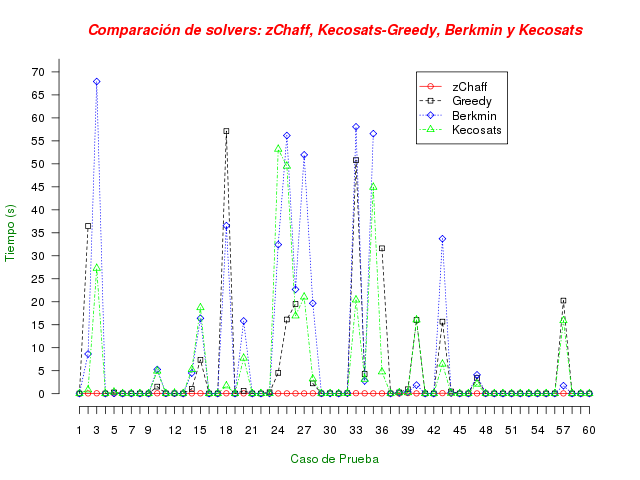
\includegraphics[scale=0.62]{tiempos_sudokuIII.png}
\end{center}

% Comentarios acerca de los resultados obtenidos, expuestos gráficamente en la
% ilustración de arriba:\vspace{-2.5mm}
% \begin{itemize}
% \item En 27 de los 60 casos de prueba (cerca del 50\% de los casos), KECOSATS
%   tiene un rendimiento \emph{ligeramente mejor} que zChaff. En estos casos, las
%   diferencias de tiempo entre KECOSATS y zChaff son algunas centésimas de
%   segundo.
% \item En 11 de los 60 casos de prueba (cerca del 15\% de los casos), KECOSATS
%   tiene un rendimiento \emph{ligeramente peor} que zChaff. En estos casos, las
%   diferencias de tiempo entre KECOSATS y zChaff son algunas centésimas de
%   segundo.
% \item En 1 de los 60 casos de prueba (cerca del 2\% de los casos), KECOSATS
%   tiene un rendimiento \emph{peor} que zChaff. En este caso, la diferencia de
%   tiempo entre KECOSATS y zChaff es de unos 45 segundos, cuando zChaff da la
%   respuesta en fracciones de segundo.
% \item En 21 de los 60 casos de prueba (cerca del 30\% de los casos), la demora
%   de KECOSATS en dar una solución es superior a los 6 min, cuando zChaff da
%   resultados en fracciones de segundo.
% \end{itemize}

\section{Conclusiones y recomendaciones}

A continuación se comentará sobre algunas recomendaciones para KECOSATS.

En esta tercera versión de KECOSATS hay varios aspectos que pudieran ser
modificados para obtener un mejor desempeño. Entre los aspectos que podemos
citar están:
\begin{itemize}
\item El manejo de la memoria. En varios puntos del programa es necesario armar
  listas de elementos y estas operaciones implican llamadas al sistema para la
  solicitud de memoria. Demás está decir el tiempo que consumen estas peticiones
  al sistema operativo. Se propone para la próxima entrega que KECOSATS
  incorpore su propio manejador de memoria, que solicite al arrancar un gran
  trozo de memoria y se encargue él solo de la gestión de este recurso,
  ahorrando así el tiempo que se consumen las llamadas {\tt malloc}. Ahora bien,
  es conocido por los desarrolladores que la realización de un manejador de
  memoria de ``buen desempeño'' no es algo trivial, particularmente si los
  segmentos de memoria que se solicitaría el programa a sí mismo pueden tener
  cualquier tamaño en algún rango dado. No obstante, dada la naturaleza de los
  elementos en las listas, los bloques de memoria que el programa se solicitaría
  a su propio manejador serían prácticamente homogéneos en cuanto al tamaño, lo
  cual facilitaría la tarea de programación de este manejador.

  Al respecto de este problema, aprovechamos de comentar que en esta tercera
  versión de KECOSATS se incluye la implementación por arreglo, de una pila de
  elementos de tipo {\tt decision\_level\_data}, que, como mencionamos en
  secciones anteriores, es el tipo de dato que almacena toda la información que
  concierne a un nivel de decisión ---la asignación de decisión y las
  asignaciones de propagación generadas por ésta, por ejemplo. Sin embargo, esta
  implementación no está integrada al resto del código, de forma que se conserva
  la implementación por listas enlazadas que se propuso en la primera versión de
  KECOSATS.

\item Los parámetros del problema de la selección de la próxima variable, al que
  nos hemos referido anteriormente en varias oportunidades. Como se ha descrito
  antes, los contadores $ac(x_i)$ tienen que ser ``envejecidos'' periódicamente
  con el fin de que los valores $ac(x_i)$ reflejen la actividad reciente. La
  manera como se efectúa este envejecimiento es la división por una constante
  pequeña. Cabe la posibilidad de variaciones en el comportamiento general del
  algoritmo para valores distintos de esta constante pequeña de
  envejecimiento. \emph{BerkMin} sugiere el valor 4, en tanto que \emph{zChaff}
  emplea el valor 2. Sería conveniente explorar con distintos valores para esta
  constante con el fin de determinar para cuál el desempeño resulta ser mejor.
  Otros parámetros al problema de la selección de variable usando la heurística
  KECOSATS, son los valores iniciales de los contadores $ac(x_i)$ ---que son 0
  para la heurística \emph{BerkMin}. Los mismos comentarios anteriores valen
  para estos parámetros también.

\item Un tercer asunto sobre el que queremos comentar es el modo en que se
  determina si una cláusula inducida por un conflicto debe ser agregada a la
  base de datos de cláusulas aprendidas. En vista de que no podemos suponer
  ilimitado el espacio disponible para aprender nuevas cláusulas, hay que ser
  selectivos con las cláusulas que se aprenden. Consideramos plausible que haya
  una heurística sencilla que determine cuáles cláusulas se descartan y cuales
  se aprenden. Ello porque podría resultar que cláusulas inducidas por conflicto
  con un tamaño superior a cierto umbral no sean tan útiles, para reducir el
  espacio de búsqueda y evitar conflictos, como cláusulas más pequeñas. Sería
  recomendable investigar sobre estas heurísticas.

\item Por último queremos mencionar acerca de los \emph{restart} o
  reinicios. Esto consiste en que llegado cierto punto en que el \emph{SAT
    solver} no ha encontrado todavía solución, éste decide descartar todas las
  asignaciones que ha hecho hasta el momento para comenzar de nuevo. Sin
  embargo, este nuevo intento de resolución del mismo problema tiene una
  diferencia con el intento que acaba de descartar: por el hecho de haber
  conservado las cláusulas que aprendió en el intento anterior, no tomará el
  mismo camino porque estas cláusulas aprendidas evitarán que vuelva a caer en
  los mismo conflictos con los que ya se había topado anteriormente. KECOSATS
  cada cierto tiempo ejecuta estos \emph{restarts} y lo que proponemos aquí como
  recomendación es probar con distintas heurísticas que ayuden a determinar
  cuándo es el momento que pareciera ser más apropiado para ejecutar estos
  reinicios.

\end{itemize}

Como conclusión de los resultados obtenidos tras la comparación de la demora de
KECOSATS y la de zChaff para resolver los 60 casos de prueba, afirmamos que el
rendimiento de la tercera versión de KECOSATS ha mejorado con respecto a la
primera y segunda versiones del programa. Observamos en esta tercera versión de
KECOSATS que el número de casos de prueba que demoraban más disminuyó
considerablemente, porque de los 21 casos de prueba ---cerca del 30\% del total
de casos--- que en la primera versión demoraban más de 6 minutos en dar
solución, sólo 3 de ellos tardaron más de ese tiempo para la segunda
versión. Para la tercera versión, no hay un caso de prueba que demore más de 54
segundos. Si sumamos los porcentajes de los números de casos que hemos
calificado con rendimientos \emph{ligeramente peores} y \emph{ligeramente
  mejores}, da 68\%. Ello quiere decir que para este porcentaje de los casos de
prueba, los rendimientos de KECOSATS y \emph{zChaff} son comparables porque las
diferencias son de a los sumo algunas centésimas de segundo.  Una vez afirmado
lo anterior, consideramos entonces que las mejoras propuestas en el apartado de
arriba merecen especial consideración, con el objetivo de disminuir los tiempos
de aquellos casos que duran más de 1 segundo.

\begin{thebibliography}{99}
\bibitem{Cook}Cook, Stephen: ``The complexity of theorem-proving
  procedures''. \emph{ACM}, 1971.
\bibitem{goldberg} Goldberg, Eugene y Novikov, Yakov: ``BerkMin: a Fast and
  Robust SAT-Solver''. \emph{Proceedings of the conference on Design, automation
    and test in Europe}, 2002.
\bibitem{Karp}Karp, Richard: ``Reducibility Among Combinatorial
  Problems''. \emph{Complexity of Computer Computations}, 1972.
\bibitem{Marques}Lynce, I. y Marques-Silva, J.: ``Efficient Data Structures for
  Fast SAT Solvers''. Reporte Técnico. \emph{Cadence European Laboratories,
    Instituto de Engenharia de Sistemas e Computadores}. 2001.
\bibitem{grasp96}Marques Silva, J. y Sakallah, Karem: ``Grasp--A New Search
  Algorithm for Satisfiability''. \emph{Proceedings of the 1996 IEEE/ACM
    international conference on Computer-aided design}, 1996.
\bibitem{YatoSeta}Yato, Takayuki y Seta, Takahiro: ``Complexity and Completeness
  of Finding Another Solution and Its Application to Puzzles''  \emph{Trans. IEICE}, E86-A(5), 2003.
\bibitem{Zhang}Zhang, Lintao y Malik, Sharad: ``The Quest for Efficient Boolean
  Satisfiability Solvers''.
\bibitem{ZhangThesis}Zhang, Lintao: ``Searching for truth: Techniques for
  satisfiability of boolean formulas''. \emph{Tesis de doctorado. Princeton
    University}. 2003.
\bibitem{url}\url{http://www.ldc.usb.ve/~meza/ci-5651/e-m2008/articulosYsoftware/FormulacionSATdeSUDOKU}
\end{thebibliography}

\end{document}
